\documentclass[jou]{apa6}

\usepackage[american]{babel}

\usepackage{csquotes}
\usepackage[style=apa,sortcites=true,sorting=nyt,backend=biber]{biblatex}
\DeclareLanguageMapping{american}{american-apa}
\addbibresource{bibliography.bib}


%%%%%%%%%%%%%%%%%%%%%%%%%%%%%%%%%%%%%%%%
%% Discrete Structures
%% The start of RBS stuff
%%%%%%%%%%%%%%%%%%%%%%%%%%%%%%%%%%%%%%%%

% Working internal and external links in PDF
\usepackage{hyperref}
% Extra math symbols in LaTeX
\usepackage{amsmath}
\usepackage{gensymb}
\usepackage{amssymb}
% Enumerations with (a), (b), etc.
\usepackage{enumerate}

\let\OLDitemize\itemize
\renewcommand\itemize{\OLDitemize\addtolength{\itemsep}{-6pt}}

\usepackage{etoolbox}
\makeatletter
\preto{\@verbatim}{\topsep=3pt \partopsep=3pt }
\makeatother

% These sizes redefine APA for A4 paper size
\oddsidemargin 0.0in
\evensidemargin 0.0in
\textwidth 6.27in
\headheight 1.0in
\topmargin -24pt
\headheight 12pt
\headsep 12pt
\textheight 9.19in



\setlength\parindent{0pt}

\title{Midterm, 2020-02-17}
\author{Discrete Structures, Fall 2020}
\affiliation{RBS}

\leftheader{Midterm, 2020-02-17}

\abstract{%
}

%\keywords{}

\begin{document}

\thispagestyle{empty}

\twocolumn
{\Large Midterm, 2020-02-17}

\vspace{6pt}
{\bf Question 1 (Boolean Expressions).}\\
Consider Boolean expression:
$$E_0 = (p \rightarrow q \rightarrow r) \wedge (q \rightarrow r \rightarrow p) \wedge (r \rightarrow p \rightarrow q)$$
\begin{center}
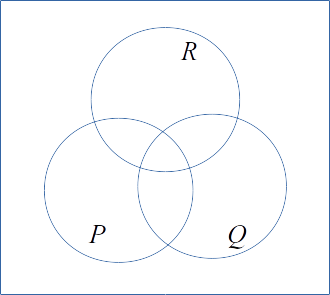
\includegraphics[width=2in]{midterm/circles.png}
\end{center}

\begin{enumerate}[(A)]
\item Copy the Venn diagram's circles in your solution and shade those regions in the diagram that make $E_0$ true
(being inside each circle $P,Q,R$ means that the respective variable $p,q,r$ is true; being outside the circle means
that the variable is false). 
\item In the truth table of $E_0$ how many entries are $\mathtt{True}$?\\
({\em Note.} Building the truth table is optional. Regardless whether you build one or not, you should justify your answer.)
\item Rewrite the Boolean expression $E_0$ into an equivalent one, using 
only conjunctions ($\wedge$) and negations ($\neg$). 
\end{enumerate}

Assume that implication ($\rightarrow$) is right-associative 
and conjunction ($\wedge$) has higher precedence than implication. 



\vspace{10pt}
{\bf Question 2 (Nested Quantifiers).}\\
Verify, if the following predicate/quantifier expressions are true for the given predicate. 
The predicate $P$ is defined on $A \times A$, where
$A = \{ \mathtt{a},\mathtt{b},\mathtt{c},\mathtt{d},\mathtt{e},\mathtt{f} \}$. 
Predicate $P(\mathtt{a},\mathtt{b})$ is true iff the square on row $\mathtt{a}$
and column $\mathtt{a}$ is shaded (and the predicate $P(\mathtt{a},\mathtt{b})$ 
is false, if that square is white).

\begin{center}
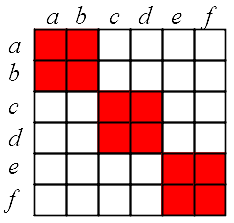
\includegraphics[width=1.2in]{midterm/relation.png}
\end{center}

\begin{enumerate}[(A)]
\item Does the predicate $P$ satisfy the logic formula:
$$\forall i \in A,\;P(i,i).$$
\item Does the predicate $P$ satisfy the logic formula:
$$\forall i \in A,\,\forall j \in A,\;P(i,j) \rightarrow P(j,i).$$
\item Does the predicate $P$ satisfy the logic formula:
$$\forall i,j,k \in A,\;P(i,j) \wedge P(j,k) \rightarrow P(i,k).$$
\item Does the predicate $P$ satisfy the logic formula:
$$\forall i,j \in A,\;P(i,j) \vee P(j,i).$$
\item Does the predicate $P$ satisfy the logic formula:
$$\forall i \in A,\, \exists j \in A,\;P(i,j).$$
\end{enumerate}

\vspace{10pt}
{\bf Question 3 (Estimate with Big-O Notation).}\\
Define the sequence $S(n)$ as a sum of squares from $1^2$ to $n^2$:
$$S(n) = \sum\limits_{i=1}^n i^2.$$
We have $S(1) = 1^2 = 1$, $S(2) = 1^2 + 2^2 = 5$, 
$S(3) = 1^2 + 2^2 + 3^2 = 14$,
and so on. 

\begin{enumerate}[(A)]
\item Is the function $S(n)$ in $O(n^1)$? 
Is it in $O(n^2)$? Is it in $O(n^3)$? Is it in $O(n^4)$? 
Explain your reasoning. 
\item Pick any one of the notations from the previous items 
($g(n)$ is either $O(n^1)$, or $O(n^2)$, or $O(n^3)$, or $O(n^4)$). 
Check the definition of Big-O notation: Find the {\em witness}: the value $k$ and the constant $C$
such that the absolute value of $S(n)$ does not exceed $C\cdot{}|g(n)|$ for all $n > k$.
\end{enumerate}


\vspace{10pt}
{\bf Question 4 (Chinese Remainder Theorem).}

Consider the following system of three congruences:
$$\left\{ \begin{array}{l}
x \equiv 1\;(\text{mod}\,5),\\
x \equiv 2\;(\text{mod}\,7),\\
x \equiv 3\;(\text{mod}\,9).
\end{array} \right.$$

\begin{enumerate}[(A)]
\item Does it have a solution? Will it have solution, even if we replace $1,2,3$ with other numbers
on the right sides of the equation.
\item Find an arithmetic progression (what is its first member $A$, difference $B$) where all members satisfy
the first two congruences from the system.
\item Find an arithmetic progression (what is its first member $C$, difference $D$) where all members satisfy
all three congruences in the system.
\end{enumerate}

{\em Note.} Arithmetic progression is an infinite sequence where every next member can be obtained
by adding the same number (the difference) to the previous one. For example, 
$$A,\;A+B,\;A+2B,\;A+3B,\ldots$$
is an arithmetic progression with the first member $A$ and the difference $B$.


\vspace{10pt}
{\bf Question 5 (Binary notation).}

Somebody has written two binary fractions on the board: $\alpha$ is infinite, $\beta$ is finite (just $6$ digits
after the point): 
$$\left\{ \begin{array}{l}
\alpha = 0.(011110)_2 = 0.011110011110011110\ldots_2\\
\beta = 0.011110_2.
\end{array} \right.$$

\begin{enumerate}[(A)]
\item Express the number $\beta$ as a sum of some negative powers of $2$; 
namely, show how to add up some of the numbers
$$\{ 2^{-1}, 2^{-2}, 2^{-3}, \ldots \}$$ 
to get $\beta$. 
\item Express $\beta$ as an irreducible fraction {\tt P/Q}; write this in the regular decimal notation. 
\item Write the product $64_{10} \cdot \alpha = 1000000_2 \cdot \alpha$ in the binary notation. 
\item Express $\alpha$ as an irreducible fraction {\tt P/Q} in decimal notation.
\end{enumerate}



\vspace{10pt}
{\bf Question 6 (Truth-tellers and Liars).}
Among the people $A,B,C$ one is a truth-teller, 
the other two are liars. 
Every person ($A$, $B$, and $C$) has a closed box
in front of himself/herself. Exactly one of the 
boxes has a candy inside. $A,B,C$ know everything 
about each other and the location of candy.

Someone else (person $D$) approaches all of them. $D$ knows, who are 
people $A$,$B$, and $C$ (it is written on their name-cards), but $D$ does
not know anything about their lying behavior or the location of the candy.
$D$ is allowed to ask YES/NO questions to one or more people.

\begin{enumerate}[(A)]
\item Can $D$ find out who has the candy by asking three questions?
\item Can $D$ find out who has the candy by asking two questions?
\item Can $D$ find out who has the candy by asking one question?
\end{enumerate}

Justify your answers (by construction or by showing that it is impossible).


\vspace{10pt}
{\bf Question 7 (Time Complexity of Truth Tables).}

Assume that there is a Boolean expression $E$ with $n$ variables: 
$$E = E(a_1,a_2,\ldots,a_n).$$
The expression $E$ contains $2n$ Boolean operators (such as $\neg$, $\wedge$, $\vee$).
Variables $a_1,a_2,\ldots,a_n$ can independently take values 
$\mathtt{True}$ or $\mathtt{False}$.

Consider the following algorithm to find, if $E$ is a tautology by 
building the truth table. We will either find a false value, or 
establish that all values were true (in this case $E$ is a tautology).

{\bf (1)} \hspace{0.0in} For each assignment of $n$ truth values to $a_1,\ldots,a_n$:\\
{\bf (2)} \hspace{0.2in} For each of the $2n$ Boolean operators in $E$:\\
{\bf (3)} \hspace{0.4in} Compute the value of that Boolean operator\\
{\bf (4)} \hspace{0.2in} If $E$ has value $\mathtt{False}$:\\
{\bf (5)} \hspace{0.4in} Return ``$E$ is not a tautology.''\\
{\bf (6)} \hspace{0.2in} If $E$ has value $\mathtt{True}$:\\
{\bf (7)} \hspace{0.4in} Continue loop on Line {\bf (1)}.\\
{\bf (8)} \hspace{0.0in} Return ``$E$ is a tautology.''

\begin{enumerate}[(A)]
\item Find the worst-case runtime $T(n)$ for this algorithm as an expression of $n$.
(Assume that evaluating one Boolean operator $\neg$, $\wedge$, $\vee$ takes $1$ unit of time.)
\item Find a function $g(n)$ such that $T(n)$ is in $O(g(n))$. 
\end{enumerate}




\vspace{10pt}
{\bf Question 8 (About Rational and Irrational).}

We denote two real numbers by $p$ and $q$. 
Prove or disprove statements about the rational and irrational numbers. 

\begin{enumerate}[(A)]
\item If $p + q$ is rational, then either both $p,q$ are rational, or both are irrational. 
\item If $pq$ is rational, then either both $p,q$ are rational, or both are irrational. 
\item If $p^2$ and $q^2$ are both rational, then the product $(p+q)(p-q)$ is rational. 
\item If $p^3$ and $p^5$ are both rational, then $p$ is rational.
\item If $pq$ and $p+q$ are both rational, then $p$ and $q$ are both rational.
\end{enumerate}

\newpage

\section{Answers}


\vspace{6pt}
{\bf Question 1}\\
{\bf (A)} The only way to have $p \rightarrow q \rightarrow r = p \rightarrow (q \rightarrow r)$ evaluate to 
$\mathtt{False}$ is $p = \mathtt{True}$ and $(q \rightarrow r) = \mathtt{False}$ (i.e.\ 
$q = \mathtt{True}$ and $r = \mathtt{False}$).\\
If we consider also $q \rightarrow r \rightarrow p$ and $r \rightarrow p \rightarrow q$, there are two 
more ways to get the whole expression $E_0$ false. Each of these ways means that exactly two variables
are $\mathtt{True}$ and the third one is $\mathtt{False}$. 
All the other areas make the expression true. Shaded areas look like this (red circles). There are just $3$ 
regions where the expression $E_0$ evaluates to false (blue letters ``F''). 
\begin{center}
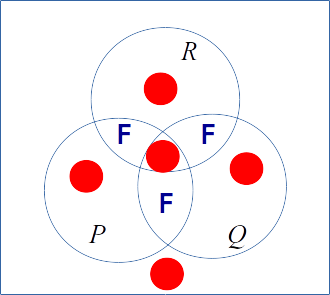
\includegraphics[width=2in]{midterm/circles-shaded.png}
\end{center}

{\bf (B)} There are exactly $8-3 = 5$ entries in the truth table which make the expression true
(there are only $3$ ways to make the expression true, as shown in {\bf (A)}). 

{\bf (C)} Let us just transform one subexpression: 
\begin{align}
 & p \rightarrow (q \rightarrow r) = \nonumber \\
= & \neg p \vee (q \rightarrow r) = \nonumber \\
= & \neg p \vee (\neg q \vee r) = \nonumber \\
= & \neg p \vee \neg q \vee r  = \nonumber \\
= & \neg (p \wedge q \wedge \neg r). \nonumber
\end{align}

If we combine all $3$ subexpressions (where $p,q,r$ switch their order), we get 
a longer conjuction for $E_0$:

$$\neg (p \wedge q \wedge \neg r) \wedge \neg (q \wedge r \wedge \neg p) \wedge \neg (r \wedge p \wedge \neg q).$$


\vspace{10pt}
{\bf Question 2}
\begin{enumerate}[(A)]
\item Yes, $\forall i \in A,\;P(i,i)$ is true (we say that the 2-argument predicate 
is {\em reflexive}): all the squares $P(i,i)$ on the diagonal of the values are shaded. 
\item Yes, $\forall i \in A,\,\forall j \in A,\;P(i,j) \rightarrow P(j,i)$ is true (we say that the 2-argument predicate 
is {\em symmetric}): the squares in the table of $P(i,j)$ are symmetric against
the diagonal of the values: $P(i,j)$ is shaded iff $P(j,i)$ is shaded.
\item Yes, $\forall i,j,k \in A,\;P(i,j) \wedge P(j,k) \rightarrow P(i,k)$ is true 
(we say that the 2-argument predicate 
is {\em transitive}). Notice that $P(i,j)$ can be true iff $i=j$ or $(i,j)$ is 
one of the pairs of neighbors: $(\mathtt{a},\mathtt{b})$, or $(\mathtt{c},\mathtt{d})$, or $(\mathtt{e},\mathtt{f})$.
$P(j,k)$ is also true; so $j,k$ also belong to the same pair. Therefore $i$ and $k$ also belong to the same pair. 
\item No, $\forall i,j \in A,\;P(i,j) \vee P(j,i)$ is false. For example, neither $P(\mathtt{a},\mathtt{c})$
nor $P(\mathtt{c},\mathtt{a})$ are true.
\item Yes, $\forall i \in A,\, \exists j \in A,\;P(i,j)$ is true: On each row $i$ there is at least
one shaded square.
\end{enumerate}


\vspace{10pt}
{\bf Question 3}
{\bf (A)} $S(n)$ is in $O(n^3)$ (and therefore it is also in $O(n^4)$). 
On the other hand, $S(n)$ is not in $O(n^2)$ or $O(n^1)$.\\
Let us show that $S(n)$ is not in $O(n^2)$. Assume from the contrary
that there are numbers $k$ and $C$ such that for each $n > k$:
$$|S(n)| = |1^2 + 2^2 + \ldots + n^2| \leq C \cdot |n^2|.$$
Since all numbers there are positive, we drop the absolute values. 
We pick any even number $n > k$ which also satisfies $n > 8C$. In this case:
\begin{align}
 & S(n) = 1^2 + 2^2 + \ldots + n^2 > \nonumber \\
> & \left( \frac{n}{2} + 1 \right)^2 + \left( \frac{n}{2} + 2 \right)^2 + \ldots + n^2 > \nonumber \\
> & \frac{n}{2} \cdot \left( \frac{n}{2} \right)^2 \geq \frac{n}{8} \cdot n^2 \geq C n^2. \nonumber 
\end{align}
{\em (In these inequalities, we first drop the first half of the sum; 
then replace each term with $(n/2)^2$ and we still can prove that the sum is more than $Cn^2$ 
for the given constant $C$.)}\\
Such $n$ can always be found (no matter what $k$ and $C$ are used). 
Therefore $S(n)$ can never satisfy $|S(n)| \leq C \cdot n^2$.\\
Since $n$ is even smaller than $n^2$, $S(n)$ is not in $O(n)$ either. 

{\bf (B)} Let us prove that $S(n)$ is in $O(n^3)$. 
Let us pick the {\em witness} to check the definition of the Big-O Notation: 
$k = 1$, $C = 1$. 
\begin{align}
     & 1^2 + 2^2 + \ldots + n^2 \leq \nonumber \\
\leq\;\; & n^2 + n^2 + \ldots + n^2=  n \cdot n^2 = 1 \cdot n^3. \nonumber
\end{align}


\vspace{10pt}
{\bf Question 4}
{\bf (A)} Yes, the system will always have solution (even if you replace the numbers $1,2,3$ by 
any other integers). Chinese Remainder theorem only needs that the modules 
($5,7,9$ in our case) are mutually prime.

{\bf (B)} The numbers satisfying $x \equiv 1\;(\text{mod}\,5)$ make this arithmetic progression: 
$$1,\,6,\,11,\,16,\,21,\,26,\,31,\,\ldots$$
Number $16$ in this progression is also congruent to $2$ (modulo $7$). The next number would be 
$16 + 35 = 51$ (because adding $5 \cdot 7 = 35$ does not change the remainders, when 
we divide by $5$ or by $7$.\\
We conclude that the following arithmetic progression satisfies the top two congruences
(remainder $1$ modulo $5$ and remainder $2$ modulo $7$):
$$16,\,51,\,86,\,121,\,156,\,191,\,\ldots$$
Answer: $A = 16$, $B = 35$. 

{\bf (C)} Observe that the first member of this arithmetic sequence ($A = 16$) gives the
remainder $7$ when divided by $9$. The difference ($B = 35$) is congruent to $8$ and also to $-1$ 
modulo $9$.\\
We conclude that by adding four differences, the result is
$$16 + 4 \cdot 35 \equiv 16 + 4 \cdot (-1) \equiv 12 \equiv 3\;(\text{mod}\,9).$$
The first number from the progression (item (B)) that is also congruent to $3$ modulo $9$ is $156$. 
We can add $5 \cdot 7 \cdot 9 = 315$ to this number, and all the remainders will stay the same:
$$156,\,471,\,786,\,1101,\,1416,\,1731,\,2046,\,\ldots$$
Answer: $C = 156$, $D = 315$.

\vspace{10pt}
{\bf Question 5}
{\bf (A)} $\beta = 0.011110_2 = 2^{-2} + 2^{-3} + 2^{-4} + 2^{-5}$.\\
{\bf (B)} $\beta = \frac{8 + 4 + 2 + 1}{2^{5}} = \frac{15}{32}$.\\
{\bf (C)} $64\alpha = 1000000_2 \cdot \alpha =$\\
$= 011110.011110011110011110\ldots_2$ (to multiply 
by $2^6 = 64$ we shift the point six positions to the right).
{\bf (D)} Subtract $\alpha$ from $64\alpha$: We get $011110_2$ (because all the 
digits after the point are the same \textendash{} they cancel out). We get the equation:
$$64\alpha - \alpha = 63\alpha = 011110_2 = 30_{10}$$
Therefore $\alpha = \frac{30}{63} = \frac{10}{21}$. We could also get the
same answer by finding the sum of an infinite geometric progression: 
$$30 \cdot \left( \frac{1}{64} + \frac{1}{64^2} + \frac{1}{64^3} + \ldots{} \right).$$


\vspace{10pt}
{\bf Question 7} 
{\bf (A)} In order to get the estimate of time complexity of the algorithm, 
consider just the first three lines, where all the computations take place:

\vspace{3pt}
{\bf (1)} \hspace{0.0in} For each assignment of $n$ truth values to $a_1,\ldots,a_n$:\\
{\bf (2)} \hspace{0.2in} For each of the $2n$ Boolean operators in $E$:\\
{\bf (3)} \hspace{0.4in} Compute the value of that Boolean operator

\vspace{3pt}
The outer loop on Line 1 repeats $2^n$ times as there are exactly $2^n$ ways to assign true/false to 
$n$ variables. The inner loop on Line 2 repeats $2n$ times (once for every operation you have to evaluate
in the expression). Line 3 takes just $1$ unit of time (this was given in the exercise). 
The time complexity $T(n)$ is the product $(2n) \cdot 2^n$; this (worst case) happens
whenever the expression is a tautology. If it is not a tautology, this algorithm will terminate earlier 
(and it will take less time). 

{\bf (B)}
This $T(n) = 2n\cdot{}2^n$ is in $O(2n\cdot{}2^n)$, since any function
is in the Big-O of itself (we can take $k = 1$ and $C = 1$). If we want, we can drop the multiplier $2$
to simplify it slightly: $T(n)$ is in $O(n\cdot{}2^n)$ (in this case $k = 1$ and $C = 2$).\\
Answer: $T(n)$ is in $O(g(n))$ where $g(n) = n\cdot{}2^n$.

\vspace{10pt}
{\bf Question 8} 
{\bf (A)} True: ``If $p + q$ is rational, then either both $p,q$ are rational, or both are irrational.''\\
From the contrary, if $p$ is rational and $q$ is irrational, then $(p + q) - p = q$ should be rational, 
which is a contradiction. Same thing happens, if $p$ is irrational and $q$ is rational. 

{\bf (B)} False: ``If $pq$ is rational, then either both $p,q$ are rational, or both are irrational.''\\
We can take $p = 0$ and $q = \sqrt{2}$; then $pq = 0$ is rational, also $p$ is rational, but $q$ is irrational. 
 
{\bf (C)} True: ``If $p^2$ and $q^2$ are both rational, then the product $(p+q)(p-q)$ is rational.''\\
Denote the two rational numbers by $\alpha = p^2$ and $\beta = q^2$. Then their difference is 
also a rational number: $\alpha - \beta = p^2 - q^2 = (p+q)(p-q)$. 

{\bf (D)} True: ``If $p^3$ and $p^5$ are both rational, then $p$ is rational.''\\
If $p = 0$ then all $p$, $p^3$ and $p^5$ are rational.\\
If $p \neq 0$, then denote the non-zero rational numbers $\alpha = p^3$ and $\beta = p^5$. 
Then their ratio $\frac{\beta}{\alpha} = \frac{p^5}{p^3} = p^2$ is also rational. 
Finally, if we divide $\alpha = p^3$ by the rational $p^2$, we get that also $p$ is rational 
(as a fraction of two rational numbers). Shortly: $p = p^1 = p^{2 \cdot 3 - 5} = \frac{ \alpha \cdot \alpha}{\beta}$. 

{\bf (E)} False: ``If $pq$ and $p+q$ are both rational, then $p$ and $q$ are both rational.''\\
Consider two irrational numbers $p = 1 + \sqrt{2}$ and $q = 1 - \sqrt{2}$. Then $p + q = 2$ and
$pq = (1 + \sqrt{2})(1 - \sqrt{2}) = 1 -2 = -1$, i.e.\ the sum and the product are both rational numbers.



\end{document}

